\documentclass{beamer}
\usepackage{natbib}
\usepackage{url}
\usepackage{stmaryrd}
\usepackage{mathrsfs}
\usepackage{amsmath}
\usepackage{graphicx}
\usepackage{parskip}
\usepackage{fancyhdr}
% \usepackage{underscore} % 下划线设置
\usepackage{commath}%定义d
\usepackage[UTF8,scheme = plain,scheme = chinese]{ctex}
\usepackage{geometry}
\usepackage{bm}
\usepackage{autobreak}
\usepackage{siunitx}
\usepackage{float}
\usepackage{subfig}
\usepackage{titlesec}
\usepackage{caption}
\usepackage{paralist}
\usepackage{multirow}
\usepackage{booktabs} % To thicken table lines
\usepackage{diagbox}
\usepackage{authblk}
\usepackage{indentfirst}
\usepackage{amsthm}
\usepackage{fontspec}
\usepackage{color}
%\usepackage{txfonts} %设置字体为times new roman
\usepackage{lettrine}
\usepackage{nameref}
%\usepackage[nottoc]{tocbibind}
\usepackage{amssymb}%font
\usepackage{lipsum}%make test words
\usepackage{picinpar}%words around the picture
\usepackage[all]{xy}%draw arrow
\usepackage{asymptote}%draw picture
\usepackage[perpage]{footmisc}%脚注每页清零
\usepackage{esint}
\renewcommand{\proofname}{\indent \sf \bfseries{证明}}

\catcode`\。=\active
\catcode`\,=\active
\catcode`\;=\active
\catcode`\:=\active
\newcommand{。}{.}
\newcommand{,}{,}
\newcommand{;}{;}
\newcommand{:}{:}

\geometry{bottom=3cm,left=3cm,right=3cm,top=3cm}
% \footskip = 60pt

% \setmainfont{TimesNewRomanPSMT}
% \setsansfont{Helvetica-Light}
% \setCJKmainfont[ItalicFont=STKaitiSC-Regular,BoldFont=STSongti-SC-Black]{STSongti-SC-Regular}
% \setCJKsansfont[BoldFont=STHeitiSC-Medium]{STHeitiSC-Light}


%\setmainfont{Times New Roman}

\ctexset{today=old}%日期类型设置

% ======================================
% = Color de la Universidad de Sevilla =
% ======================================
\usepackage{tikz}
\definecolor{PKUred}{cmyk}{0,1,1,0.45}

%超链接设置
\usepackage[breaklinks,colorlinks,linkcolor=PKUred,citecolor=PKUred,pagebackref,urlcolor=PKUred]{hyperref}
\usepackage{cleveref}
\newcommand{\crefpairconjunction}{ 和 }

% 节样式设置
% \newcommand{\hsp}{\hspace{20pt}}
% \newcommand{\nhsp}{\hspace{-30pt}}
% \titleformat{\section}{\Large\bfseries}{%\arabic{section}
%   \hspace{-22pt}\textcolor{PKUred}{\vrule width 2pt}\hsp}{0pt}{}


\titleformat{\subsection}
{\normalfont\large\bfseries}{}{0em}{}

% footnote 设置
% \renewcommand*\footnoterule{%
%   \vspace*{-3pt}%
%   {\color{PKUred}\hrule width 2in height 0.4pt}%
%   \vspace*{2.6pt}%
% }


%% Color the bullets of the itemize environment and make the symbol of the third
%% level a diamond instead of an asterisk.
%h\renewcommand*\textbullet{\dag}
\renewcommand*\labelitemi{\color{PKUred}\textbullet}
\renewcommand*\labelitemii{\color{PKUred}--}
\renewcommand*\labelitemiii{\color{PKUred}$\diamond$}
\renewcommand*\labelitemiv{\color{PKUred}\textperiodcentered}



%%% Equation and float numbering
\numberwithin{equation}{section}		% Equationnumbering: section.eq#
\numberwithin{figure}{section}			% Figurenumbering: section.fig#
\numberwithin{table}{section}				% Tablenumbering: section.tab#


%代码设置
\usepackage{listings}
\usepackage{fontspec} % 定制字体
% \newfontfamily\menlo{SFMono-Regular}
\usepackage{xcolor} % 定制颜色
\definecolor{mygreen}{rgb}{0,0.6,0}
\definecolor{mygray}{rgb}{0.5,0.5,0.5}
\definecolor{mymauve}{rgb}{0.58,0,0.82}
\lstset{
    numbers=left,
    numberstyle=\footnotesize\ttfamily,
    basicstyle=\footnotesize\ttfamily,
    backgroundcolor=\color{white},      % choose the background color
    columns=fullflexible,
    tabsize=4,
    breaklines=true,               % automatic line breaking only at whitespace
    captionpos=b,                  % sets the caption-position to bottom
    commentstyle=\color{mygreen},  % comment style
    escapeinside={\%*}{*)},        % if you want to add LaTeX within your code
    keywordstyle=\color{blue},     % keyword style
    stringstyle=\color{mymauve}\ttfamily,  % string literal style
    frame=single,
    rulesepcolor=\color{red!20!green!20!blue!20},
    % identifierstyle=\color{red},
    language=c++,
    xleftmargin=4em,xrightmargin=2em, aboveskip=1em,
    framexleftmargin=2em,
    numbers=left
}

% 脚注
% \renewcommand\thefootnote{\fnsymbol{footnote}}

%定义常数i、e、积分符号d
\newcommand\mi{\mathrm{i}}
\newcommand\me{\mathrm{e}}

%%% Maketitle metadata
\newcommand{\horrule}[1]{\rule{\linewidth}{#1}} 	% Horizontal rule
\newcommand{\tabincell}[2]{\begin{tabular}{@{}#1@{}}#2\end{tabular}}



\usetheme[progressbar=frametitle]{metropolis}

\setsansfont{TimesNewRomanPSMT}
\setmonofont{SFMono-Regular}
\setmainfont{TimesNewRomanPSMT}

\title{\LaTeX 极速入门}
\institute{北京大学工学院}
\author{袁磊祺}
\date{\today}
%\logo{
\includegraphics[width=5em]{pkured.pdf}}

\setCJKsansfont[ItalicFont=STKaitiSC-Regular,BoldFont=STSongti-SC-Black]{STSong}
\setCJKmainfont[BoldFont=STHeitiSC-Medium]{STHeitiSC-Light}

\catcode`\。=\active
\catcode`\,=\active
\catcode`\;=\active
\catcode`\:=\active
\newcommand{。}{.}
\newcommand{,}{,}
\newcommand{;}{;}
\newcommand{:}{:}


\begin{document}
\maketitle
\begin{frame}
  \frametitle{Outlines}
  \tableofcontents{}
\end{frame}
\section{\LaTeX 简介}
\begin{frame}[allowframebreaks]{\TeX 历史}
  \begin{enumerate}
    \item  \TeX(/tɛx/,常被读作/tɛk/,音译“泰赫”,“泰克”,写作“TEX”),是一个由美国计算机教授高德纳(Donald Ervin Knuth)编写的排版软件。它在学术界特别是数学、物理学和计算机科学界十分流行。高德纳在 看到其 巨 著 “The Art of Computer Programming”第二卷的校样时, 对排版的低质量感到无法忍受,于是决 定开发一个高质量的计算机排版系统\TeX .
    \item \LaTeX(/ˈlɑːtɛks/,常被读作/ˈlɑːtɛk/或/ˈleɪtɛk/,写作“\LaTeX”),是一种基于 \TeX 的排版系统,由美国计算机科学家莱斯利·兰伯特在20世纪80年代初期开发.
    \item XeTeX(/ˈziːtɛx/或/ˈziːtɛk/,文本模式下写作XeTeX)是一种使用Unicode的TeX排版引擎,并支持一些现代字体技术.
  \end{enumerate}

  \begin{figure}[h]
    \centering
    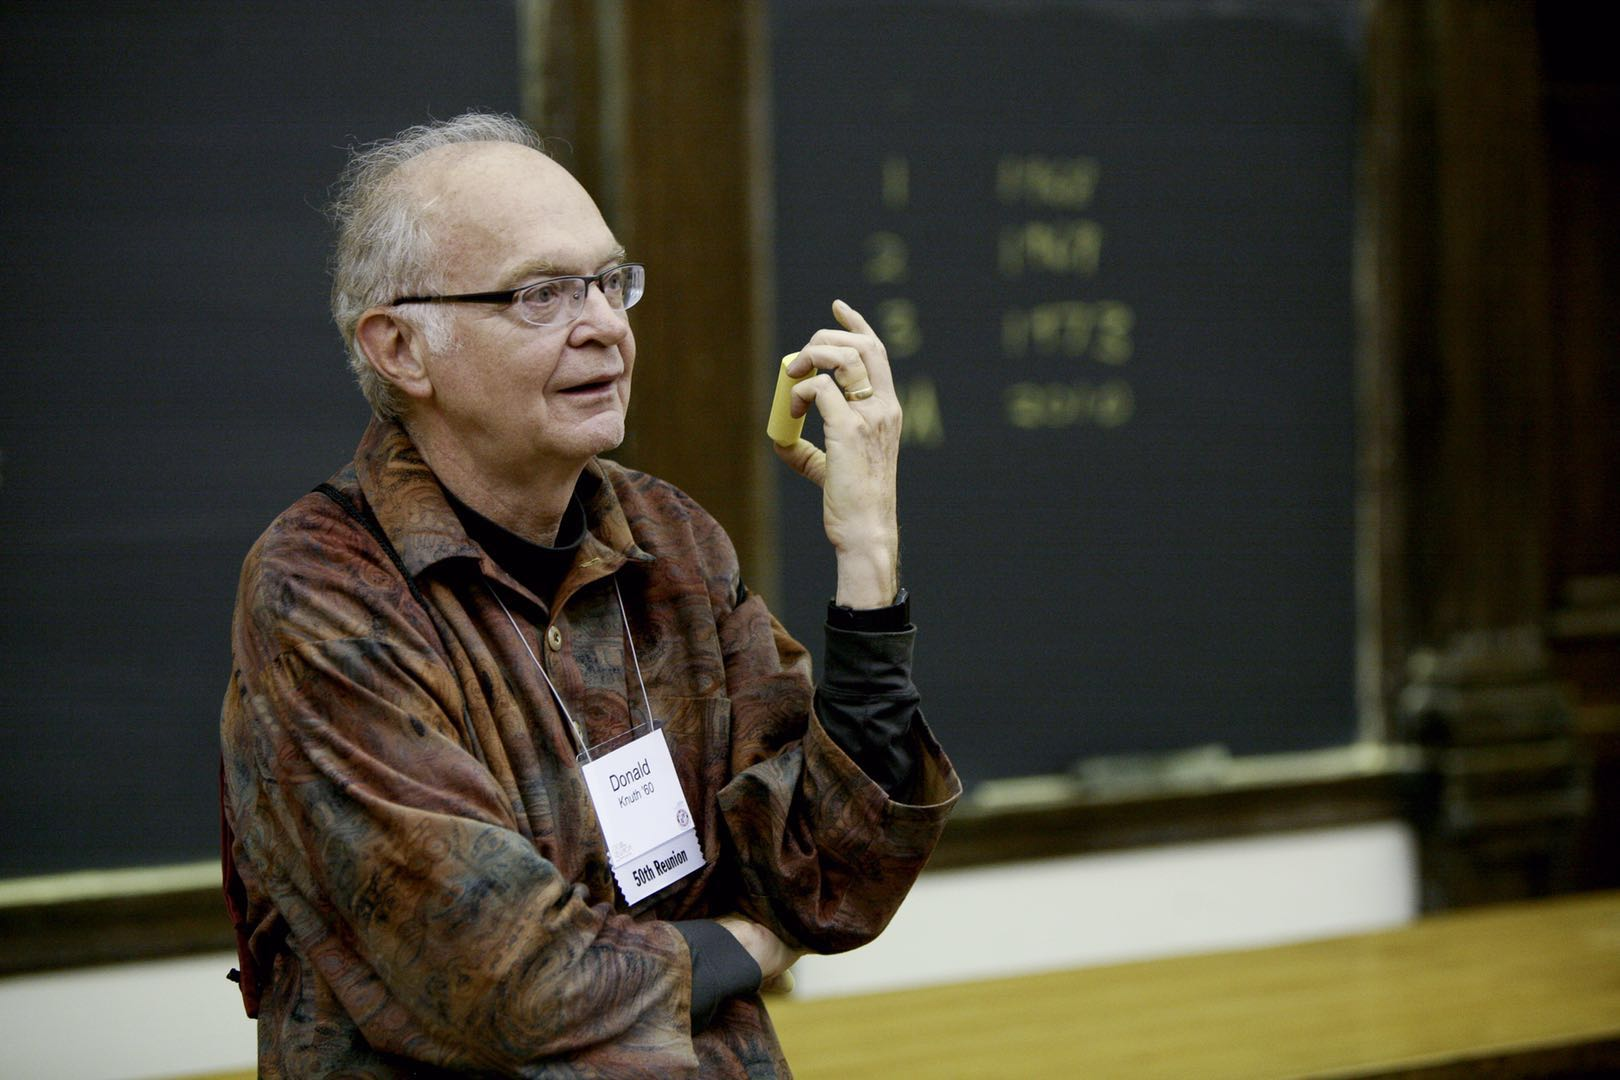
\includegraphics[width=8cm]{Knuth.jpeg}
    \caption{D. E. Knuth.}
    \label{fig:Knuth}
  \end{figure}

\end{frame}

\begin{frame}{\LaTeX\  IDE}
  \begin{itemize}
    \item<1-> Overleaf
    \begin{itemize}
      \item[-] 在线编辑;
      \item[-] 团队合作;
      \item[-] 模版丰富;
      \item[*] 速度较慢;
      \item[*] 高级功能收费。
    \end{itemize}
    \item<2-> \TeX\  live + VScode + GitHub(推荐)
    \begin{itemize}
      \item[-] 功能全面,没有的功能可以通过配置完善。
    \end{itemize}
  \end{itemize}
\end{frame}

\begin{frame}{推荐资料}
  网上搜索某个功能$\to$找到要用的包$\to$看这个包的说明文档。

  见最后的参考文献第 \ref{page:ref} 页。
  \label{page:1}
\end{frame}

\begin{frame}[fragile,allowframebreaks]{Hello, World!}

  注释:以 \% 开头至行尾,如 \verb|% this is a comment|.

  命令:以 \verb|\| 开头,如:
  \begin{lstlisting}[language=tex]
\command % a command
\command{} % also a command
\command{arg} % a command with an argument
\command{arg1}{arg2} 
% a command with multiple arguments 
\command[opt]{arg} % [] is for optional argument
\end{lstlisting}
  可使用 \verb|\newcommand{cmd}[args][opt]{def}|
  命令定义新命令,或使用\verb|\renewcommand{cmd}[args][opt]{def}| 重写已有命令的定义。

  环境:由\verb|\begin{} ... \end{}|包裹,如:
  \begin{lstlisting}
\begin{envname}
% inside the environment
\end{envname}
% LaTeX environment can take arguments 
\begin{envname}{arg}   ... \end{envname} 
\begin{envname}[opt]{arg} ... \end{envname}
\end{lstlisting}
\end{frame}


\section{文章结构}

\begin{frame}[fragile]{Hello, World!}
  新建名为 hello-world.tex 的文件:
  \begin{lstlisting}[language=tex]
\documentclass{article}
\title{First {\LaTeX} Document} 
\author{Circle} 
\date{\today}
\begin{document} 
\maketitle 
Hello, world! 
\end{document}
\end{lstlisting}

\end{frame}

\begin{frame}[fragile]{\LaTeX 文件结构}
  \verb|\begin{document} ... \end{document}|之 间 的 部 分 为 文 档 内 容, 可以:
  \begin{itemize}
    \item 使用 \verb|\maketitle| 命令自动生成标题。
    \item 使用 \verb|\tableofcontents| 命令自动生目录。
    \item 使用 \verb|\chapter{} / \section{} / \subsection{}| 命令完成文档的章 节结构排版和用于自动生成目录。
    \item 使用 \verb|figure / table / equation| 等环境在文档中插入对应的元素。 使用 \verb|\label{} / \ref{} / \cref{}| 命令处理交叉引用。
  \end{itemize}
  最后 \LaTeX 文件以 \verb|\end{document}| 结尾。

\end{frame}

\begin{frame}[fragile]{多文件编辑}
  使用  \verb|\input{file.tex}| 命令,可以将\verb|setting.tex|文件内容在该命 令处展开.

  类似于 C 语言中的\verb|#include "setting.h"|宏指令。
\end{frame}

\section{公式}

\begin{frame}{公式}
  \begin{figure}[htp]
    \centering
    
\includegraphics[width=3cm]{mathpix.jpg}
    \caption{\href{https://mathpix.com}{Mathpix}}
    \label{fig:Mathpix}
  \end{figure}

\end{frame}

\section{图片}

\begin{frame}[fragile]{图片}

  上一张图的代码:
  \begin{lstlisting}[language=tex]
\begin{figure}[htp]
  \centering
  
\includegraphics[width=3cm]{mathpix.jpg}
  \caption{\href{https://mathpix.com}{Mathpix}}
  \label{fig:Mathpix}
\end{figure}
\end{lstlisting}

\end{frame}

\section{表格}

\begin{frame}[fragile]{表格}

  \begin{table}[htp]
    \centering
    \caption{表格示例.}
    \begin{tabular}{cc}
      \toprule  1 & 2     \\
      \midrule
      内容1       & 内容2 \\
      \bottomrule
    \end{tabular}
    \label{tab:1}
  \end{table}

  \begin{lstlisting}[language=tex]
  \begin{table}[htp]
    \centering
    \caption{表格示例.}
    \begin{tabular}{cc}
      \toprule  1 & 2  \\
          \midrule
      内容1 & 内容2\\
      \bottomrule
    \end{tabular}
    \label{tab:1}
  \end{table}
\end{lstlisting}

\end{frame}

\section{参考文献}

\begin{frame}[fragile]{参考文献}

  $\mathrm{XeLaTeX}\to \mathrm{BiBTeX}\to \mathrm{XeLaTeX}\to \mathrm{XeLaTeX}$.

  \verb|.bib| 文件:
  \begin{lstlisting}[language=tex]
@book{texbook,
author = {Knuth, Donald Ervin},
date-added = {2021-05-02 18:50:03 +0800},
date-modified = {2021-05-02 18:50:55 +0800},
publisher = {Addison-Wesley Pub. Co.},
title = {The TeXbook},
year = {c1984}}
\end{lstlisting}

\end{frame}

\begin{frame}[allowframebreaks]{References}
  回到第 \ref{page:1} 页。
  \label{page:ref}
  \nocite{*}
  \bibliography{ppt}
  \bibliographystyle{abbrv}

\end{frame}

\end{document}





